\documentclass[12pt,a4paper]{article}

% --------------------
% Pacotes básicos
% --------------------
\usepackage[utf8]{inputenc}   % Codificação de caracteres
\usepackage[T1]{fontenc}      % Acentuação correta
\usepackage[brazil]{babel}    % Idioma português
\usepackage{geometry}         % Controle de margens
\usepackage{hyperref}         % Links clicáveis no PDF
\usepackage{setspace}         % Espaçamento
\usepackage{enumitem}         % Personalização de listas
\usepackage{graphicx}         % Para inserir imagens

% --------------------
% Configurações
% --------------------
\geometry{a4paper, margin=2.5cm}
\setstretch{1.2} % Espaçamento 1.5
\hypersetup{
    colorlinks=true,
    linkcolor=blue,
    urlcolor=blue,
    citecolor=blue
}
\setlist{nosep} % Listas mais compactas

% --------------------
% Início do documento
% --------------------
\begin{document}

\title{Projeto de Engenharia de Software \\ \large Sistema de Gestão dos Restaurantes Universitários da UFF}
\author{
    Aluno 1 \\ 
    Aluno 2 \\ 
    Aluno 3 \\ 
    Aluno 4 \\ 
    Aluno 5 \\ 
    Aluno 6 \\ 
    Aluno 7 \\ 
    Aluno 8 \\ 
    Aluno 9
}
\date{\today}

\maketitle

\tableofcontents
\newpage

% --------------------
% Seção: Escopo
% --------------------
\section{Escopo}

\subsection{Nome provisório do projeto}
Sistema de Gestão dos Restaurantes Universitários da UFF (SG-RU/UFF).



\subsection{Descrição}
Desenvolver e operar um sistema integrado para os Restaurantes Universitários (RUs) da UFF em Niterói que gerencie:
\begin{enumerate}
    \item Fila virtual de acesso;
    \item Estoque de insumos e refeições prontas;
    \item Logística entre unidades;
    \item Cardápio e informações nutricionais.
\end{enumerate}
O sistema terá interfaces para perfis administrativos e será acessível aos usuários finais (discentes, docentes e servidores) através do aplicativo IdUFF.

% --------------------
% Seção: Requisitos Funcionais
% --------------------
\section{Requisitos Funcionais}

\subsection{Requisitos Gerais}
\begin{enumerate}[label=\textbf{RF-GEN-\arabic*}, leftmargin=*, align=left]
    \item \textbf{Autenticação via IdUFF (SSO).} O sistema deve permitir login do usuário utilizando o SSO institucional (IdUFF), garantindo sessão segura e expiração configurável. % (equivale ao rf1.1)

    \item \textbf{Interfaces por perfil.} O sistema deve exibir interfaces distintas para: (a) administradores/operadores do RU e (b) usuários finais (discentes, docentes e servidores) que utilizam o RU. % (equivale ao rf1.2)

    \item \textbf{Níveis de acesso (RBAC).} O sistema deve suportar perfis e papéis com permissões diferenciadas (por exemplo: Administrador, Operador de Cozinha, Logística, Nutrição/Qualidade, Usuário Final), restringindo ações e telas conforme o papel. % (equivale ao rf1.3)

    
\end{enumerate}

\subsection{Requisitos da Fila para Usuários}
\begin{enumerate}[label=\textbf{RF-FIL-U-\arabic*}, leftmargin=*, align=left]
    \item O sistema deve possuir um sistema de fila virtual associado ao ingresso no RU.
    \item O sistema deve permitir que o usuário entre na fila virtual.
    \item O sistema deve permitir que o usuário saia da fila virtual.
    \item O sistema deve exibir ao usuário sua posição atual na fila.
    \item O sistema deve notificar o usuário sobre a evolução de sua posição na fila.
    \item O sistema deve permitir que o usuário personalize suas preferências de notificação (ex.: push, frequência).
    \item O sistema deve permitir diferentes níveis de prioridade ao entrar na fila, conforme políticas institucionais (idosos, PCDs, bolsistas, etc.).
    \item O sistema deve exibir ao usuário uma estimativa de tempo de espera (ETA).
    \item O sistema deve exibir avisos ao usuário em caso de imprevistos operacionais no RU (ex.: atrasos, falta de energia).
    \item O sistema deve permitir que o usuário confirme ou desista de sua posição na fila quando solicitado.
    \item O sistema deve oferecer a possibilidade de o usuário retroceder voluntariamente posições na fila.
    \item O sistema deve permitir que os usuários enviem feedbacks sobre a experiência na fila virtual.
\end{enumerate}

\subsection{Requisitos da Fila para Administradores}
\begin{enumerate}[label=\textbf{RF-FIL-A-\arabic*}, leftmargin=*, align=left]
    \item O sistema deve exibir em tempo real o número de pessoas na fila, o tempo médio de espera e os horários de pico.
    \item O sistema deve receber informações das catracas físicas presentes no local para registrar pessoas entrando e saindo do RU.
    \item O sistema deve permitir que os administradores monitorem quantas pessoas estão simultaneamente no refeitório.
    \item O sistema deve controlar a capacidade máxima de pessoas simultaneamente no refeitório, bloqueando novas entradas quando necessário.
    \item O sistema deve gerar relatórios históricos de fluxo de pessoas e de refeições servidas.
  
    \item O sistema deve permitir a gestão e configuração das regras de prioridade de entrada (idosos, gestantes, PCDs, bolsistas, etc.).
\end{enumerate}


\subsection{Requisitos de Estoque}
\begin{enumerate}[label=\textbf{RF-EST-\arabic*}, leftmargin=*, align=left]
    \item O sistema deve armazenar a quantidade de ingredientes em estoque.
    \item O sistema deve armazenar a quantidade de alimentos prontos para consumo em estoque.
    \item O sistema deve permitir que o administrador edite a quantidade de ingredientes em estoque.
    \item O sistema deve permitir que o administrador edite a quantidade de alimentos prontos para consumo em estoque.
    \item O sistema deve permitir que o administrador consulte a quantidade de cada ingrediente não preparado.
    \item O sistema deve permitir que o administrador consulte a quantidade de cada alimento pronto para consumo.
    \item O sistema deve permitir que o administrador informe quando um certo item, em um determinado RU, acabou.
    \item O sistema deve permitir que o administrador faça um pedido de envio de mais comida.
    \item O sistema deve notificar o responsável pelo envio de comida sobre os pedidos recebidos.
    \item O sistema deve permitir que o administrador responsável pelo envio receba feedback do pedido realizado.
    \item O sistema deve possibilitar que os administradores monitorem as informações da viagem de envio (tempo estimado, item pedido, veículo de transporte, motorista responsável).
    \item O sistema deve permitir que o administrador registre relatórios de consumo de ingredientes e refeições em diferentes períodos (diário — almoço/janta, semanal, mensal).
    \item O sistema deve permitir que o administrador registre eventuais sobras de comida.
    \item O sistema deve emitir alertas quando o estoque mínimo de um ingrediente for atingido.
    \item O sistema deve permitir que o administrador consulte o prazo de validade de cada ingrediente.
\end{enumerate}

\subsection{Requisitos de Receitas e Nutrição}
\begin{enumerate}[label=\textbf{RF-NUT-\arabic*}, leftmargin=*, align=left]
    \item O sistema deve conter um processo de aprovação do controle de qualidade dos alimentos.
    \item O sistema deve exibir ao usuário o cardápio do dia.
    \item O sistema deve possibilitar ao usuário o acesso às informações nutricionais dos alimentos.
    \item O sistema deve permitir que funcionários do RU registrem casos de contaminação de alimentos.
    \item O sistema deve alertar os funcionários responsáveis pela gestão do RU em casos de contaminação dos alimentos.
    \item O sistema deve permitir que o usuário avalie a qualidade da refeição recebida.
    \item O sistema deve permitir que o administrador informe os valores nutricionais de cada alimento.
    \item O sistema deve gerar relatórios nutricionais consolidados (por exemplo: média de calorias e nutrientes ofertados por semana).
\end{enumerate}

\section{Requisitos Não-Funcionais}

\subsection{Requisitos Gerais}
\begin{enumerate}[label=\textbf{RNF-GEN-\arabic*}, leftmargin=*, align=left]
    \item O sistema deve seguir diretrizes de acessibilidade digital WCAG 2.1, garantindo que pessoas com deficiência possam utilizá-lo (ex.: contraste adequado, navegação por teclado, leitores de tela).
\end{enumerate}

\subsection{Requisitos de Fila}
\begin{enumerate}[label=\textbf{RNF-FIL-\arabic*}, leftmargin=*, align=left]
    \item O sistema deve atualizar a posição do usuário na fila em intervalos de no máximo 60 segundos.
    \item O sistema deve permanecer disponível durante todo o horário de funcionamento das refeições (mínimo de 2h15 a partir do início de cada turno), com disponibilidade mínima de 99\% no período crítico.
\end{enumerate}

\subsection{Requisitos de Estoque}
\begin{enumerate}[label=\textbf{RNF-EST-\arabic*}, leftmargin=*, align=left]
    \item O sistema deve atualizar a quantidade de ingredientes em estoque em tempo real, com base nas baixas de preparação registradas.
    \item O sistema deve ser capaz de suportar múltiplos acessos simultâneos (administradores, cozinha, nutricionista), garantindo consistência dos dados.
    \item O sistema deve proteger dados sensíveis (como custos e fornecedores) por meio de autenticação e controle de permissões baseado em papéis (RBAC).
\end{enumerate}

\subsection{Requisitos de Receitas e Nutrição}
\begin{enumerate}[label=\textbf{RNF-NUT-\arabic*}, leftmargin=*, align=left]
    \item O sistema deve exibir o cardápio e as informações nutricionais em até 2 segundos após a solicitação.
    \item As avaliações de usuários sobre qualidade da refeição devem ser armazenadas de forma segura, protegidas contra acesso não autorizado.
\item As avaliações de usuários sobre qualidade da refeição devem:
\begin{itemize}
    \item ser registradas apenas por usuários autenticados;
    \item ser armazenadas de forma a garantir sua integridade (sem alteração não autorizada);
    \item ser acessíveis apenas a administradores e nutricionistas, não sendo exibidas publicamente com identificação pessoal do avaliador.
\end{itemize}

\end{enumerate}


\section{Casos de Uso}

\subsection{Fila}

\subsubsection{UC-FILA-01 — Entrar na fila}
\textbf{Atores:} Usuário autenticado (via IdUFF).  

\textbf{Fluxo principal:}
\begin{enumerate}
    \item O usuário acessa o sistema IdUFF.
    \item O usuário abre a tela da fila e seleciona o RU desejado.
    \item O sistema exibe capacidade e tamanho da fila, bem como regras/políticas.
    \item O usuário (se elegível) escolhe a prioridade desejada.
    \item O usuário confirma a entrada na fila.
    \item O sistema valida a elegibilidade (RU aberto, critérios atendidos, etc.).
    \item O sistema registra o ingresso e atribui posição.
    \item O sistema calcula e apresenta a estimativa de espera (ETA).
    \item O sistema agenda as notificações conforme preferências do usuário.
\end{enumerate}

\textbf{Cenários alternativos:}
\begin{itemize}
    \item \textbf{2.a: RU fechado ou indisponível} — O sistema informa indisponibilidade e retorna ao passo 1.
    \item \textbf{4.a: Usuário não elegível à prioridade} — O sistema oculta opções de prioridade e retorna ao passo 4.
    \item \textbf{4.b: Validação manual de prioridade} — O usuário envia foto de comprovante; o sistema valida e retorna ao passo 4.
    \item \textbf{5.a: Saldo insuficiente} — O sistema recusa a entrada na fila e informa necessidade de regularização via IdUFF; após ajuste, retorna ao passo 5.
\end{itemize}

% ----------------------------------------------------------------
\subsubsection{UC-FILA-02 — Sair da fila (Desistência)}
\textbf{Atores:} Usuário autenticado.  

\textbf{Fluxo principal:}
\begin{enumerate}
    \item O usuário aciona a opção “Sair da fila”.
    \item O sistema solicita confirmação.
    \item O usuário confirma.
    \item O sistema remove o usuário e reordena a fila.
    \item O sistema atualiza ETA dos demais e confirma a saída.
    \item O sistema registra, opcionalmente, o motivo da desistência.
\end{enumerate}

\textbf{Cenários alternativos:}
\begin{itemize}
    \item \textbf{2.a: Usuário muito próximo de ser chamado} — O sistema informa política de desistência; o usuário confirma e segue ao passo 4 ou cancela e retorna ao passo 1.
\end{itemize}

% ----------------------------------------------------------------
\subsubsection{UC-FILA-03 — Consultar posição e ETA}
\textbf{Atores:} Usuário autenticado.  

\textbf{Fluxo principal:}
\begin{enumerate}
    \item O usuário abre a tela da fila no IdUFF.
    \item O sistema exibe posição atual, ETA e avisos do RU.
    \item O sistema atualiza automaticamente em intervalos definidos.
    \item O usuário pode solicitar atualização manual.
\end{enumerate}

\textbf{Cenários alternativos:}
\begin{itemize}
    \item \textbf{1.a: Usuário não está na fila} — O sistema oferece ação “Entrar na fila”; se aceito, executa UC-FILA-01.
    \item \textbf{2.a: Imprevistos no RU} — O sistema recalcula ETA, exibe aviso e retorna ao passo 2.
\end{itemize}

% ----------------------------------------------------------------
\subsubsection{UC-FILA-04 — Configurar notificações}
\textbf{Atores:} Usuário autenticado.  

\textbf{Fluxo principal:}
\begin{enumerate}
    \item O usuário abre a tela da fila pelo IdUFF.
    \item O usuário acessa “Preferências de notificação”.
    \item O usuário define limiares (ex.: faltam X pessoas/minutos).
    \item O sistema valida configurações e salva.
    \item O sistema confirma a ativação das preferências.
\end{enumerate}

% ----------------------------------------------------------------
\subsubsection{UC-FILA-05 — Confirmar presença}
\textbf{Atores:} Usuário autenticado.  

\textbf{Fluxo principal:}
\begin{enumerate}
    \item O sistema dispara um prompt de confirmação ao atingir um marco (ex.: top 50/top 20).
    \item O usuário confirma presença.
    \item O sistema mantém a posição e registra o timestamp.
\end{enumerate}

\textbf{Cenários alternativos:}
\begin{itemize}
    \item \textbf{2.a: Sem resposta no prazo} — O sistema remove o usuário da fila por inatividade e notifica a remoção.
    \item \textbf{2.b: Usuário escolhe desistir} — O sistema executa UC-FILA-02.
\end{itemize}

% ----------------------------------------------------------------
\subsubsection{UC-FILA-06 — Retroceder posições}
\textbf{Atores:} Usuário autenticado.  

\textbf{Fluxo principal:}
\begin{enumerate}
    \item O usuário abre a tela da fila pelo IdUFF.
    \item O usuário seleciona “Retroceder”.
    \item O sistema solicita a matrícula do usuário alvo.
    \item O usuário confirma a operação.
    \item O sistema altera a posição e reordena a fila.
    \item O sistema recalcula o ETA e confirma nova posição.
\end{enumerate}

\textbf{Cenários alternativos:}
\begin{itemize}
    \item \textbf{3.a: Matrícula inválida} — O sistema retorna erro e volta ao passo 3.
    \item \textbf{4.a: Limite excedido} — O sistema informa a regra e bloqueia a operação, retornando ao passo 2.
\end{itemize}

% ----------------------------------------------------------------
\subsubsection{UC-FILA-07 — Enviar feedback da experiência}
\textbf{Atores:} Usuário autenticado.  

\textbf{Fluxo principal:}
\begin{enumerate}
    \item O sistema oferece formulário curto após atendimento ou desistência.
    \item O usuário avalia tempo/organização/satisfação e insere comentários.
    \item O sistema registra o feedback e apresenta agradecimento.
\end{enumerate}

\textbf{Cenários alternativos:}
\begin{itemize}
    \item \textbf{1.a: Usuário ignora a solicitação} — O sistema não insiste e encerra o fluxo.
\end{itemize}

% ----------------------------------------------------------------
\subsubsection{UC-FILA-08 — Ver painel em tempo real (Admin)}
\textbf{Atores:} Administrador.  

\textbf{Fluxo principal:}
\begin{enumerate}
    \item O administrador acessa o painel.
    \item O sistema exibe pessoas na fila, ETA médio e horários de pico.
    \item O administrador aplica filtros (turno, campus, período).
\end{enumerate}

\textbf{Cenários alternativos:}
\begin{itemize}
    \item \textbf{2.a: Dados de catraca indisponíveis} — O sistema sinaliza degradação e utiliza dados estimados.
\end{itemize}

% ----------------------------------------------------------------
\subsubsection{UC-FILA-09 — Configurar capacidade e prioridades (Admin)}
\textbf{Atores:} Administrador.  

\textbf{Fluxo principal:}
\begin{enumerate}
    \item O administrador abre “Configurações de operação”.
    \item O sistema valida permissões de acesso.
    \item O administrador define a capacidade simultânea.
    \item O administrador configura critérios de prioridade e pesos.
    \item O administrador define abertura/fechamento do RU.
    \item O sistema valida consistência e salva.
    \item O sistema aplica as regras ao motor de fila e recalcula ETA.
\end{enumerate}

\textbf{Cenários alternativos:}
\begin{itemize}
    \item \textbf{2.a: Nível de acesso insuficiente} — O sistema bloqueia a operação e retorna à tela inicial.
\end{itemize}

% ----------------------------------------------------------------
\subsubsection{UC-FILA-10 — Conciliar eventos das catracas}
\textbf{Atores:} Administrador, Sistema de catracas.  

\textbf{Fluxo principal:}
\begin{enumerate}
    \item A catraca envia evento de entrada/saída.
    \item O sistema registra o evento e atualiza contagem.
    \item O sistema cruza eventos com a fila (chamados vs. entrados).
    \item O sistema sinaliza divergências e gera lista de conferência.
\end{enumerate}

\textbf{Cenários alternativos:}
\begin{itemize}
    \item \textbf{1.a: Falha de comunicação} — O sistema enfileira eventos e sinaliza degradação.
    \item \textbf{3.a: Divergência persistente} — O sistema gera ticket para verificação manual.
\end{itemize}

% ----------------------------------------------------------------
\subsubsection{UC-FILA-11 — Gerar relatórios (Admin)}
\textbf{Atores:} Administrador.  

\textbf{Fluxo principal:}
\begin{enumerate}
    \item O administrador solicita relatório.
    \item O administrador escolhe período e indicadores.
    \item O sistema consolida dados de fila, catracas e feedbacks.
    \item O sistema apresenta visualização e permite download.
\end{enumerate}

\textbf{Cenários alternativos:}
\begin{itemize}
    \item \textbf{3.a: Volume de dados elevado} — O sistema avisa sobre maior tempo de processamento e sugere filtros.
\end{itemize}

\subsection{Estoque}

\subsubsection{UC-ESTOQUE-01 — Preparo da comida}
\textbf{Atores:} Responsável pela retirada (RPR).  

\textbf{Visão geral:} Preparar alimentos para consumo, dando baixa em insumos e atualizando o estoque de refeições prontas.  

\textbf{Referência cruzada:} RF-EST-1, RF-EST-2, RF-EST-3, RF-EST-4, RF-EST-5, RF-EST-6, RF-EST-7, RF-EST-14.  

\textbf{Pré-condição:} Há insumos necessários em estoque.  

\textbf{Pós-condição:} Insumos são reduzidos e quantidade de comida pronta é atualizada.  

\textbf{Fluxo principal:}
\begin{enumerate}
    \item O responsável retira a quantidade necessária de insumos.
    \item O responsável dá baixa no estoque.
    \item O sistema chama UC-ESTOQUE-07 (Atualizar estoque de insumos).
    \item O sistema atualiza a quantidade de alimentos prontos.
    \item Os cozinheiros preparam a comida.
\end{enumerate}

\textbf{Cenários alternativos:}
\begin{itemize}
    \item \textbf{3.a: Limite mínimo identificado} — O sistema alerta (RF-EST-14); o responsável notifica compras. Retorna ao passo 4.
    \item \textbf{5.a: Erro no preparo} — A comida é descartada; fluxo retorna ao passo 1.
\end{itemize}

% -----------------------------------------------------------
\subsubsection{UC-ESTOQUE-02 — Envio da comida}
\textbf{Atores:} RU remetente e RU destinatário.  

\textbf{Visão geral:} O RU remetente envia refeições prontas a outro RU, com baixa no estoque e notificação.  

\textbf{Referência cruzada:} RF-EST-4, RF-EST-6, RF-EST-11.  

\textbf{Pré-condição:} Há comida pronta suficiente em estoque.  

\textbf{Pós-condição:} Estoque atualizado e RU destinatário notificado.  

\textbf{Fluxo principal:}
\begin{enumerate}
    \item O responsável consulta a quantidade solicitada.
    \item O responsável retira a quantidade do estoque.
    \item O responsável dá baixa no estoque.
    \item O sistema atualiza registros.
    \item O responsável registra as informações do pedido.
    \item O responsável confirma a saída da comida.
    \item O sistema notifica o RU destinatário.
    \item Chama UC-ESTOQUE-04 (Receber comida).
\end{enumerate}

% -----------------------------------------------------------
\subsubsection{UC-ESTOQUE-03 — Pedido de comida}
\textbf{Atores:} RU destinatário e RU fornecedor.  

\textbf{Visão geral:} Um RU solicita mais comida a outro.  

\textbf{Referência cruzada:} RF-EST-4, RF-EST-6, RF-EST-7, RF-EST-8, RF-EST-9, RF-EST-10.  

\textbf{Pré-condição:} RU destinatário precisa de comida adicional.  

\textbf{Pós-condição:} Pedido aceito ou recusado.  

\textbf{Fluxo principal:}
\begin{enumerate}
    \item O RU destinatário envia solicitação.
    \item O RU fornecedor recebe notificação.
    \item O RU fornecedor aceita o pedido.
    \item O sistema notifica o RU destinatário da aceitação.
    \item Chama UC-ESTOQUE-02 (Envio da comida).
\end{enumerate}

\textbf{Cenários alternativos:}
\begin{itemize}
    \item \textbf{3.a: Pedido negado} — O RU fornecedor recusa e notifica; o RU destinatário recebe negativa; fluxo encerrado.
\end{itemize}

% -----------------------------------------------------------
\subsubsection{UC-ESTOQUE-04 — Receber comida}
\textbf{Atores:} RU fornecedor e RU destinatário.  

\textbf{Visão geral:} O RU destinatário recebe, confere e atualiza o estoque de refeições prontas.  

\textbf{Referência cruzada:} RF-EST-4, RF-EST-6, RF-EST-8, RF-EST-10.  

\textbf{Pré-condição:} Envio concluído e registrado.  

\textbf{Pós-condição:} Estoque do RU destinatário atualizado.  

\textbf{Fluxo principal:}
\begin{enumerate}
    \item O RU destinatário confere a comida recebida.
    \item O RU destinatário notifica recebimento.
    \item O RU fornecedor recebe confirmação.
    \item O RU destinatário atualiza estoque no sistema.
\end{enumerate}

\textbf{Cenários alternativos:}
\begin{itemize}
    \item \textbf{1.a: A comida não chegou} — O RU destinatário registra divergência; chama UC-ESTOQUE-03.
    \item \textbf{1.b: Quantidade insuficiente} — O RU destinatário registra divergência; pode solicitar o restante; chama UC-ESTOQUE-03.
\end{itemize}

% -----------------------------------------------------------
\subsubsection{UC-ESTOQUE-05 — Gerar relatório}
\textbf{Atores:} Supervisor.  

\textbf{Visão geral:} O supervisor solicita relatórios personalizados de consumo e estoque.  

\textbf{Referência cruzada:} RF-EST-12, RF-EST-15.  

\textbf{Pré-condição:} Há dados suficientes.  

\textbf{Pós-condição:} Relatório gerado e exibido.  

\textbf{Fluxo principal:}
\begin{enumerate}
    \item O supervisor escolhe parâmetros.
    \item O supervisor solicita relatório.
    \item O sistema consolida dados.
    \item O sistema exibe relatório e permite download.
\end{enumerate}

\textbf{Cenários alternativos:}
\begin{itemize}
    \item \textbf{3.a: Erro de consolidação} — O sistema notifica erro; fluxo encerrado.
\end{itemize}


% -----------------------------------------------------------
\subsubsection{UC-ESTOQUE-06 — Fim de serviço}
\textbf{Atores:} Supervisor.  

\textbf{Visão geral:} O supervisor atualiza o sistema com a quantidade de refeições que sobraram ao final do expediente.  

\textbf{Referência cruzada:} RF-EST-12, RF-EST-13.  

\textbf{Pré-condição:} O horário de funcionamento do RU chegou ao fim.  

\textbf{Pós-condição:} É registrado no sistema a informação sobre a quantidade de comida que sobrou.  

\textbf{Fluxo principal:}
\begin{enumerate}
    \item O responsável registra o encerramento do serviço no sistema.
    \item O responsável informa a quantidade de comida pronta que sobrou.
    \item O sistema atualiza os registros de estoque com os valores informados.
\end{enumerate}

% -----------------------------------------------------------
\subsubsection{UC-ESTOQUE-07 — Atualizar estoque de insumos}
\textbf{Atores:} Administrador ou responsável pelo estoque.  

\textbf{Visão geral:} O sistema atualiza o estoque de insumos em função de entradas ou saídas (uso em preparo ou recebimento de novos insumos).  

\textbf{Referência cruzada:} RF-EST-1, RF-EST-3, RF-EST-5.  

\textbf{Gatilho:} UC-ESTOQUE-01 (Preparo da comida) ou UC-ESTOQUE-08 (Receber insumos).  

\textbf{Pré-condição:} Há movimentação de insumos (entrada ou saída).  

\textbf{Pós-condição:} Quantidade final de insumos refletida corretamente no estoque.  

\textbf{Fluxo principal:}
\begin{enumerate}
    \item O sistema identifica movimentação (entrada ou saída de insumos).
    \item O sistema calcula a nova quantidade de insumos.
    \item O sistema atualiza o estoque com o valor corrigido.
\end{enumerate}

% -----------------------------------------------------------
\subsubsection{UC-ESTOQUE-08 — Receber insumos}
\textbf{Atores:} Responsável pelo recebimento (RU remetente).  

\textbf{Visão geral:} O RU recebe insumos, contabiliza as quantidades e atualiza o sistema.  

\textbf{Referência cruzada:} RF-EST-1, RF-EST-3, RF-EST-5.  

\textbf{Pré-condição:} Há novos insumos entregues ao RU.  

\textbf{Pós-condição:} A quantidade final de insumos em estoque é incrementada corretamente.  

\textbf{Fluxo principal:}
\begin{enumerate}
    \item Os insumos chegam ao RU.
    \item O responsável contabiliza a quantidade recebida.
    \item O sistema chama UC-ESTOQUE-07 (Atualizar estoque de insumos).
\end{enumerate}

\subsection{Receitas e Nutrição}

\subsubsection{UC-NUTRI-01 — Aprovação do controle de qualidade}
\textbf{Atores:} Administrador.  

\textbf{Referência cruzada:} RF-NUT-1.  

\textbf{Pré-condição:} Administrador logado no sistema.  

\textbf{Fluxo principal:}
\begin{enumerate}
    \item A equipe de controle de qualidade vai ao local de preparo.
    \item A equipe averigua o estado da comida.
    \item O administrador aprova a qualidade da comida no sistema.
    \item O sistema registra a aprovação.
    \item O sistema exibe ao administrador o status da aprovação.
\end{enumerate}

\textbf{Cenários alternativos:}
\begin{itemize}
    \item \textbf{2.a: A comida não passa pelo controle de qualidade}  
    \begin{enumerate}
        \item O administrador reprova a comida no sistema.
        \item O sistema registra a reprovação.
        \item O sistema notifica supervisores responsáveis sobre o incidente.
        \item O sistema exibe ao administrador o status da reprovação.
        \item Fim do caso de uso.
    \end{enumerate}
\end{itemize}

% -----------------------------------------------------------
\subsubsection{UC-NUTRI-02 — Consulta do cardápio}
\textbf{Atores:} Cliente.  

\textbf{Referência cruzada:} RF-NUT-2, RF-NUT-3.  

\textbf{Fluxo principal:}
\begin{enumerate}
    \item O cliente acessa a área de cardápio do dia.
    \item O sistema lista todos os restaurantes abertos.
    \item O cliente seleciona um restaurante.
    \item O sistema exibe o cardápio do dia incluindo informações nutricionais.
\end{enumerate}

\textbf{Cenários alternativos:}
\begin{itemize}
    \item \textbf{1.a: Cliente não está conectado} — Caso de uso incluído: Login.
\end{itemize}

% -----------------------------------------------------------
\subsubsection{UC-NUTRI-03 — Relatar contaminação}
\textbf{Atores:} Funcionário.  

\textbf{Referência cruzada:} RF-NUT-4, RF-NUT-5.  

\textbf{Pré-condição:} Funcionário logado no sistema; caso de contaminação identificado.  

\textbf{Fluxo principal:}
\begin{enumerate}
    \item O funcionário acessa a área “Relatos de contaminação”.
    \item O sistema exibe formulário.
    \item O funcionário descreve o ocorrido.
    \item O funcionário envia o relato.
    \item O sistema registra o relato.
    \item O sistema notifica supervisores.
\end{enumerate}

% -----------------------------------------------------------
\subsubsection{UC-NUTRI-04 — Registrar valores nutricionais}
\textbf{Atores:} Administrador.  

\textbf{Referência cruzada:} RF-NUT-7.  

\textbf{Pré-condição:} Administrador logado no sistema.  

\textbf{Fluxo principal:}
\begin{enumerate}
    \item O administrador acessa a seção de alimentos.
    \item O sistema exibe os alimentos registrados.
    \item O administrador inicia edição de um alimento.
    \item O sistema exibe as informações do alimento.
    \item O administrador edita as informações nutricionais.
    \item O administrador finaliza alterações.
    \item O sistema salva as mudanças.
\end{enumerate}

% -----------------------------------------------------------
\subsubsection{UC-NUTRI-05 — Acessar relatórios nutricionais consolidados}
\textbf{Atores:} Administrador.  

\textbf{Referência cruzada:} RF-NUT-8.  

\textbf{Pré-condição:} Administrador logado no sistema.  

\textbf{Fluxo principal:}
\begin{enumerate}
    \item O administrador acessa a seção de relatórios nutricionais.
    \item O sistema gera relatório consolidado com base nos cardápios semanais.
    \item O sistema exibe o relatório para o administrador.
\end{enumerate}

% Adicione esta seção após os Casos de Uso e antes do \end{document}

\section{Diagramas}

\subsection{Diagrama Geral de Casos de Uso}

A Figura~\ref{fig:diagrama_geral} apresenta a visão geral do sistema, mostrando todos os atores e casos de uso principais dos três módulos integrados: Fila Virtual, Estoque e Receitas/Nutrição.

\begin{figure}[htbp]
    \centering
    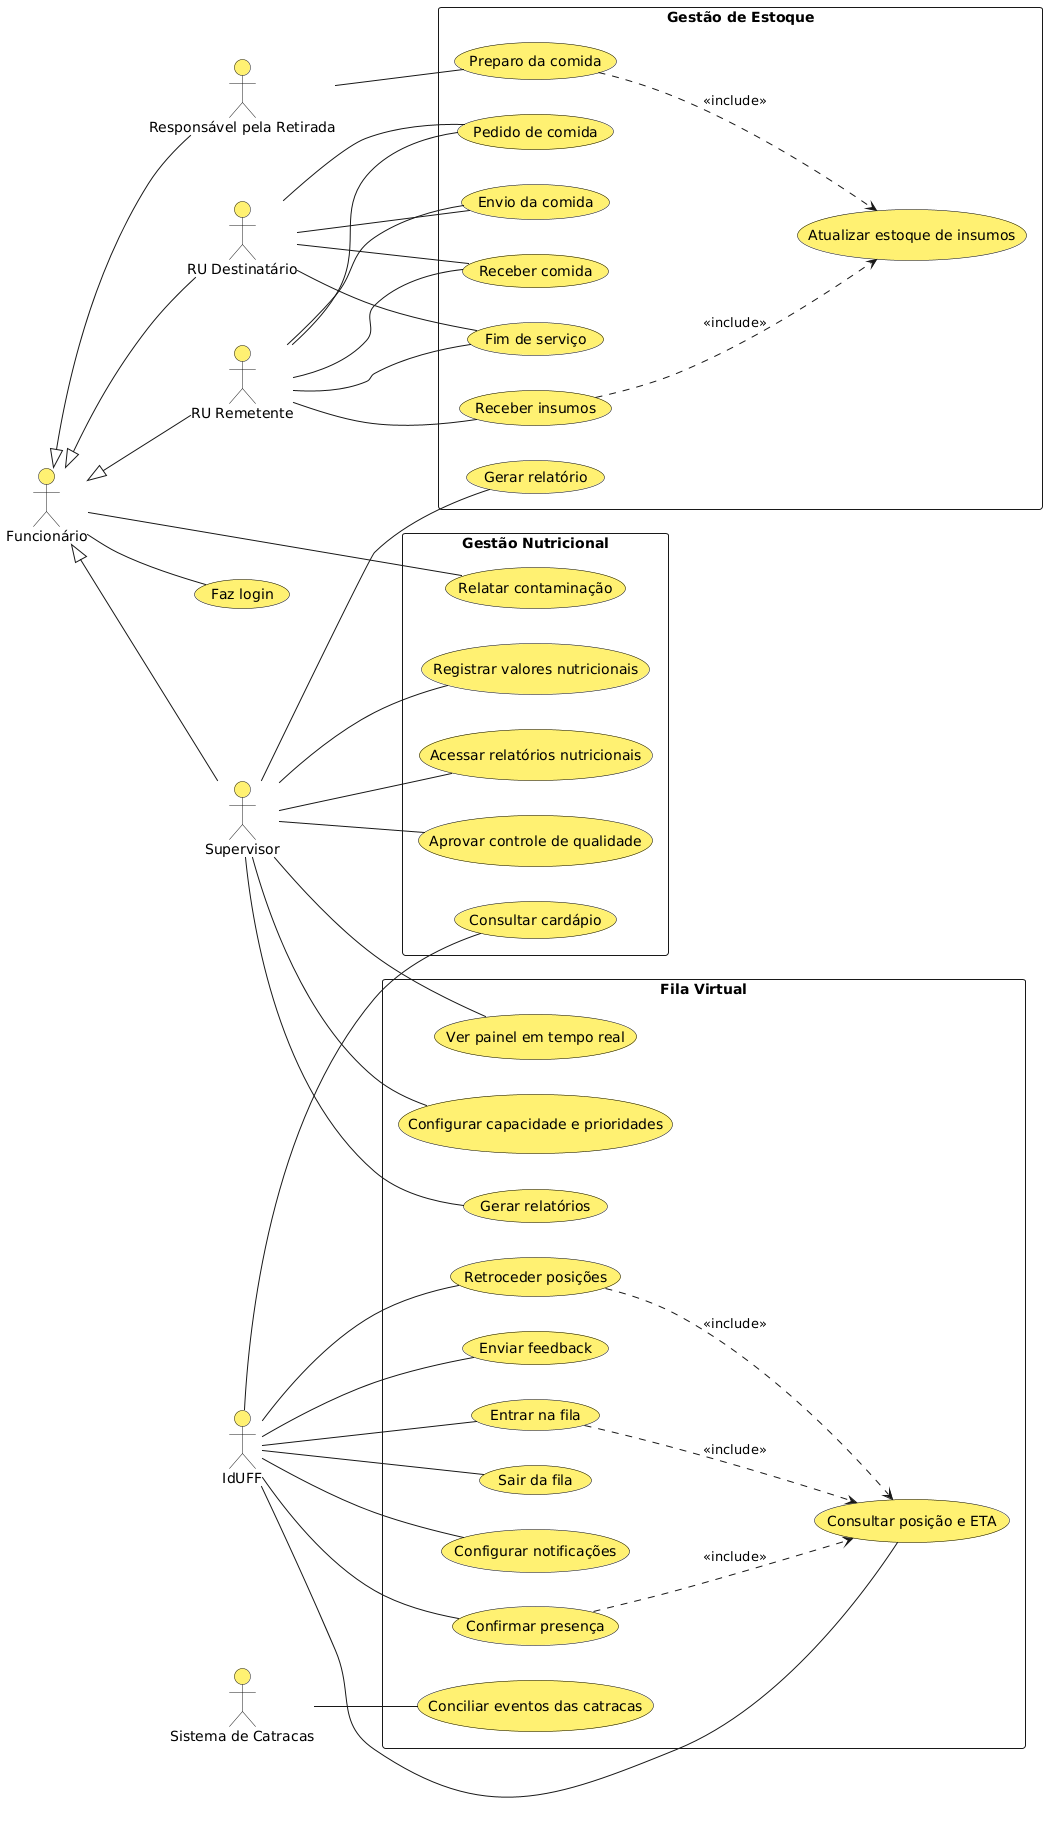
\includegraphics[width=0.9\textwidth]{diagramas/diagrama-geral.png}
    \caption{Diagrama geral de casos de uso do Sistema de Gestão dos RUs da UFF}
    \label{fig:diagrama_geral}
\end{figure}

O diagrama ilustra as interações entre os diferentes perfis de usuários (Usuário Final, Administrador, Funcionário, Nutricionista) e as principais funcionalidades do sistema, demonstrando a integração entre os módulos de gestão.

\subsection{Diagramas por Módulo}

\subsubsection{Módulo Fila Virtual}
A Figura~\ref{fig:diagrama_fila} detalha os casos de uso específicos do módulo de fila virtual.

\begin{figure}[htbp]
    \centering
    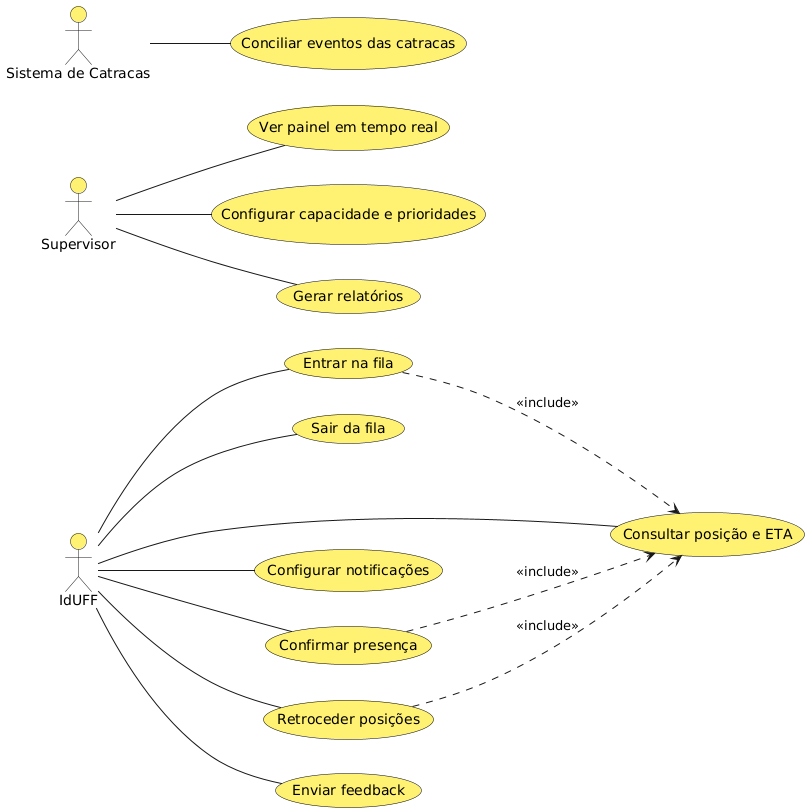
\includegraphics[width=0.8\textwidth]{diagramas/diagrama-fila.png}
    \caption{Diagrama de casos de uso - Módulo Fila Virtual}
    \label{fig:diagrama_fila}
\end{figure}

\subsubsection{Módulo Estoque}
A Figura~\ref{fig:diagrama_estoque} apresenta os casos de uso do módulo de gestão de estoque.

\begin{figure}[htbp]
    \centering
    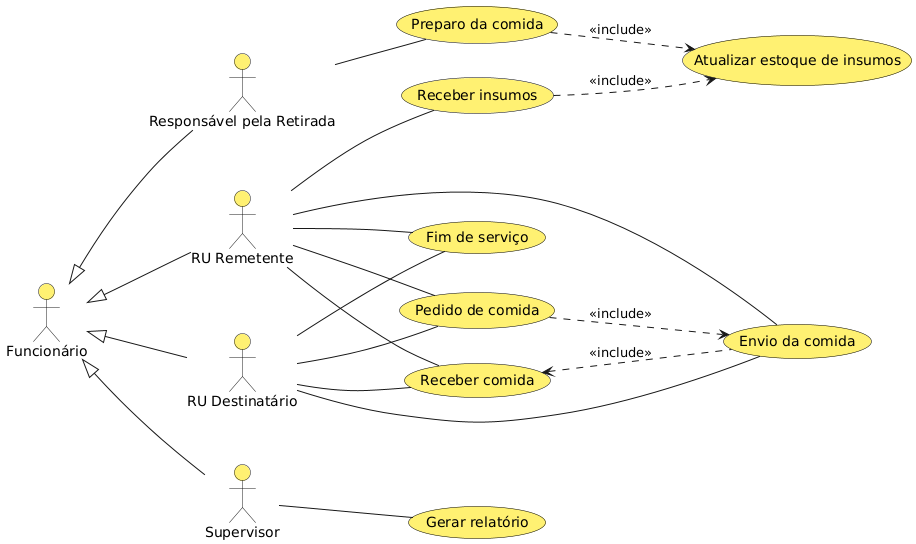
\includegraphics[width=0.8\textwidth]{diagramas/diagrama-estoque.png}
    \caption{Diagrama de casos de uso - Módulo Estoque}
    \label{fig:diagrama_estoque}
\end{figure}

\subsubsection{Módulo Receitas e Nutrição}
A Figura~\ref{fig:diagrama_nutricao} ilustra os casos de uso relacionados à gestão nutricional.

\begin{figure}[htbp]
    \centering
    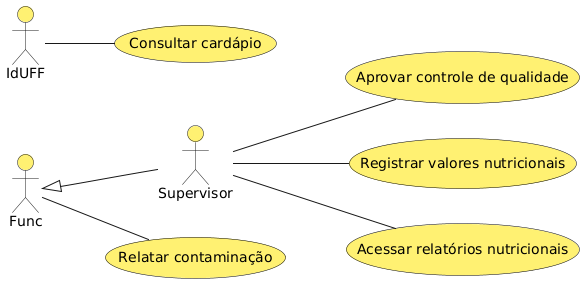
\includegraphics[width=0.8\textwidth]{diagramas/diagrama-nutricao.png}
    \caption{Diagrama de casos de uso - Módulo Receitas e Nutrição}
    \label{fig:diagrama_nutricao}
\end{figure}

\end{document}
